\chapter{Linear Time Reversal}
\label{ch:ltr}

\section{Purpose}
\label{sec:ltr-purpose}

In investigating the applicability of time reversal to a wireless power transfer system, there are several properties that we would like to characterize further. While transferring a meaningful amount of energy to a receiver is the primary goal, but there are other characteristics to consider as well. We are interested in the ability to select a receiver to send energy to, while minimizing the wasted energy that is sent to other locations. We are interested in being able to transmit energy to a receiver in a complex environment, which may have an obstructed line of sight. We are interested in transferring power to a receiver in motion. We are interested in the range over which we can efficiently transfer power. How does TR perform in these capabilities? In this section, we investigate two of these characteristics.

Of first importance is the transferring meaningful amounts of power. Here, "meaningful" is a relative term; depending on the application and what is being powered with the WPT scheme, the demand for energy will vary. The amount of energy required to charge an electric car (on the order of 3 kW) will be vastly larger than the amount of energy required to charge a mobile phone (on the order of 10 W), for example. ~\cite{witricity2013subsea} Our target application is the charging of cell phones, so it is necessary to investigate how much power can be transmitted safely using TR. For this specific WPT technique, this translates into the size and frequency of pulses that can be sent to the receiver.

We also would like to characterize the extent to which TR can be used to charge a receiver in motion. Motion of either the receiver or transmitter is a limitation of many WPT technologies; we ask if TR is also subject to this limitation. Time reversal research has focused primarily on the technique's use in stationary environments with stationary transducers. Some research has shown that TR can be used as a motion detector, relying on the destruction of TR fidelity correlated with a change in the environment. ~\cite{taddese_sensing_2010} However, we would like to investigate the effect of small receiver position changes on the TR process. 

Understanding these phenomena allows us to make a judgement on whether TR could be used as an effective WPT technique. If TR can transmit large amounts of energy to a receiver, it fulfills the primary goal of a WPT scheme and merits further examination. Consideration of the more advanced goal of sending energy to a receiver in motion is more detailed. This ability is a gap in the current market, and is not prominent in current WPT technologies. Having identified this shortcoming, TR can fulfill a need that is not currently being met if it is able to target a receiver in motion.

\section{Methodology for Conducting Linear Time Reversal Measurements}
\label{sec:ltr-meth}

We conducted physical experiments to answer the following questions:
\begin{itemize}
    \item What modifications will allow TR send a meaningful amount of power to a receiver?
    \item How can TR be used to target receivers in motion?
\end{itemize}
Both of these proposals require similar methodologies for investigation. As such, the experiments we conducted shared much of the same equipment and procedure. Here we will detail the process that we used for establishing a linear time reversal mirror between two ports.

These experiments take place within an enclosed, reflective cavity called a "gigabox" for ease of reference: an aluminum box with a metallic foil scattering paddle to make the ray trajectories more ergodic. The resulting ray chaos ensures that a propagating waveform will eventually reach every point in the environment. This is essential for the proper function of a time reversal mirror. Up to five identical monopole antennas can inject and extract electromagnetic signals from different ports in the enclosure, but for these experiments only two were used. One antenna was held stationary, while the other was mounted on a scanning window that could acommodate motion of up to 70 millimeters in one dimension. Ports on opposing sides of the gigabox were selected to avoid confounding short orbit effects which result from an insufficient mode density between the injecting and receiving ports.

Our time reversal scheme consists of several pieces of microwave processing equipment and a desktop workstation. Interrogation pulses and time-reversed sona signals are created and broadcast using a Tektronix \texttt{AWG7052} arbitrary waveform generator feeding an Agilent \texttt{E8267D} Vector PSG microwave source. A digital storage oscilloscope (DSO, Agilent \texttt{DSO91304A}) is used to record waveforms of interest. MATLAB version 2015a is used for signal processing, instrument control and coordination. Connections between the microwave equipment and the gigabox antennas are made using standard coaxial cables.

In many experiments, it is necessary to be able to ``read'' and ``write'' signals from the same port. Manually switching coaxial cables from the PSG to the DSO is slow and can destroy reconstructions, so we use four HP 8762C coaxial switches to reroute signals as required. The relative connections of the hardware are laid out in Figure~\ref{fig:linear-gigabox}.

\begin{figure}[h!]
\centering
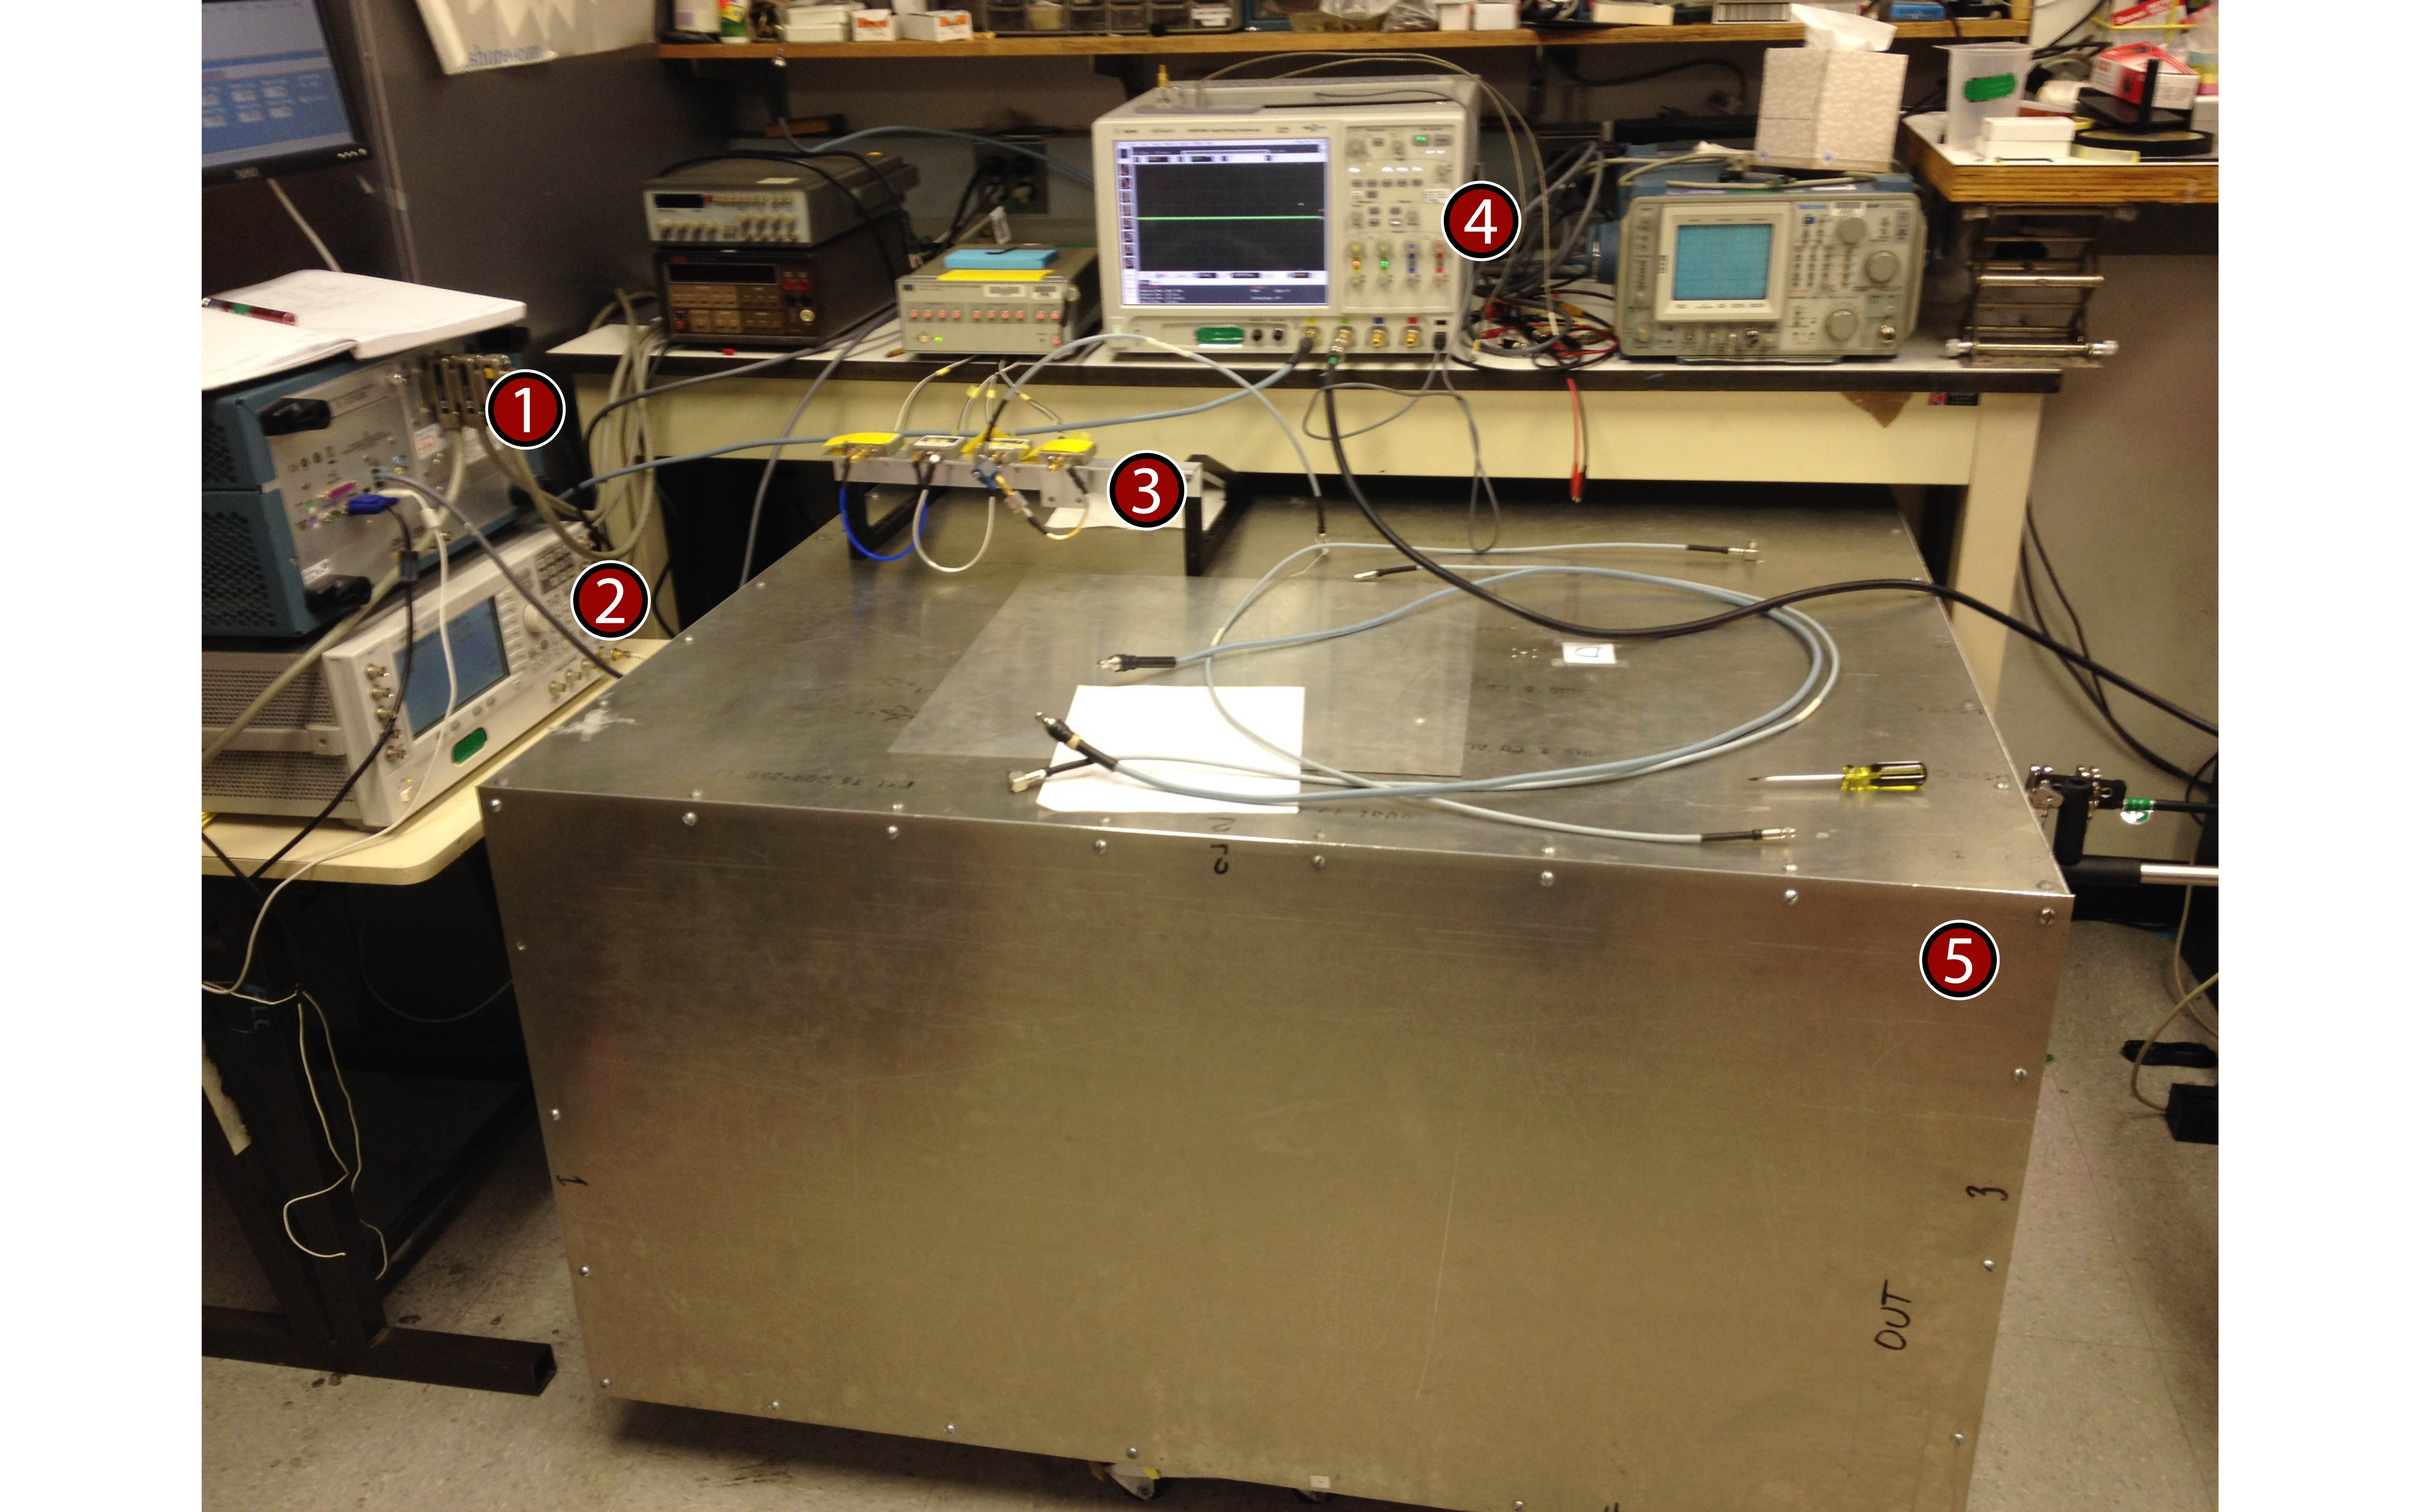
\includegraphics[width=0.85\textwidth]{linear/gigabox}
    \caption[Experimental Setup]{Experimental setup used: (1) Tektronix \texttt{AWG7052} Arbitrary Waveform Generator, (2) Agilent \texttt{E8267D} Vector PSG Microwave Source, (3) Array of four Hewlett-Packard 8762C coaxial switches, (4) Agilent \texttt{DSO91304A} Digital Storage Oscilloscope, 5) 1.06~$m^3$ aluminum ``Gigabox'' with interior conductive scattering paddle.}
    \label{fig:linear-gigabox}
\end{figure}

TR processes fall into two main categories, linear and nonlinear. Linear TR (LTR) refers to any experiment that uses a single frequency for the interrogation pulse, time reversed sona, and reconstruction. Nonlinear TR (NLTR) makes use of harmonic reflections from the target to provide a means for isolation and targeting, a process similar to how we would envision a TR based WPT system to work.  It is experimentally much simpler to create reconstructions with LTR than with NLTR. For this reason, these experiments are conducted in the absence of nonlinear elements which respond to a fundamental frequency by generating harmonic signals at a variety of frequencies. 

Conceptually, our general process for LTR in the Gigabox is as follows: we broadcast a Gaussian interrogation pulse from one port, serving as a transmitter. This interrogation pulse reverberates and echoes around the reflective cavity. Another port, designated as the receiver, records the multipath sum of these reverberations with the oscilloscope. This summed signal is named a sona, and inherently contains information relating to the size and shape of the interrogation pulse, the location of any scattering media in the environment, and the location of both ports. That sona is reversed in the time domain and subsequently rebroadcast from the transmitting port. The signal will travel through the same multipath channels and reconstruct a time reversed version of the original interrogation pulse upon the receiver, with some additional noise. This process is illustrated in Figure~\ref{fig:linear-ltr}.

\begin{figure}[h!]
\centering
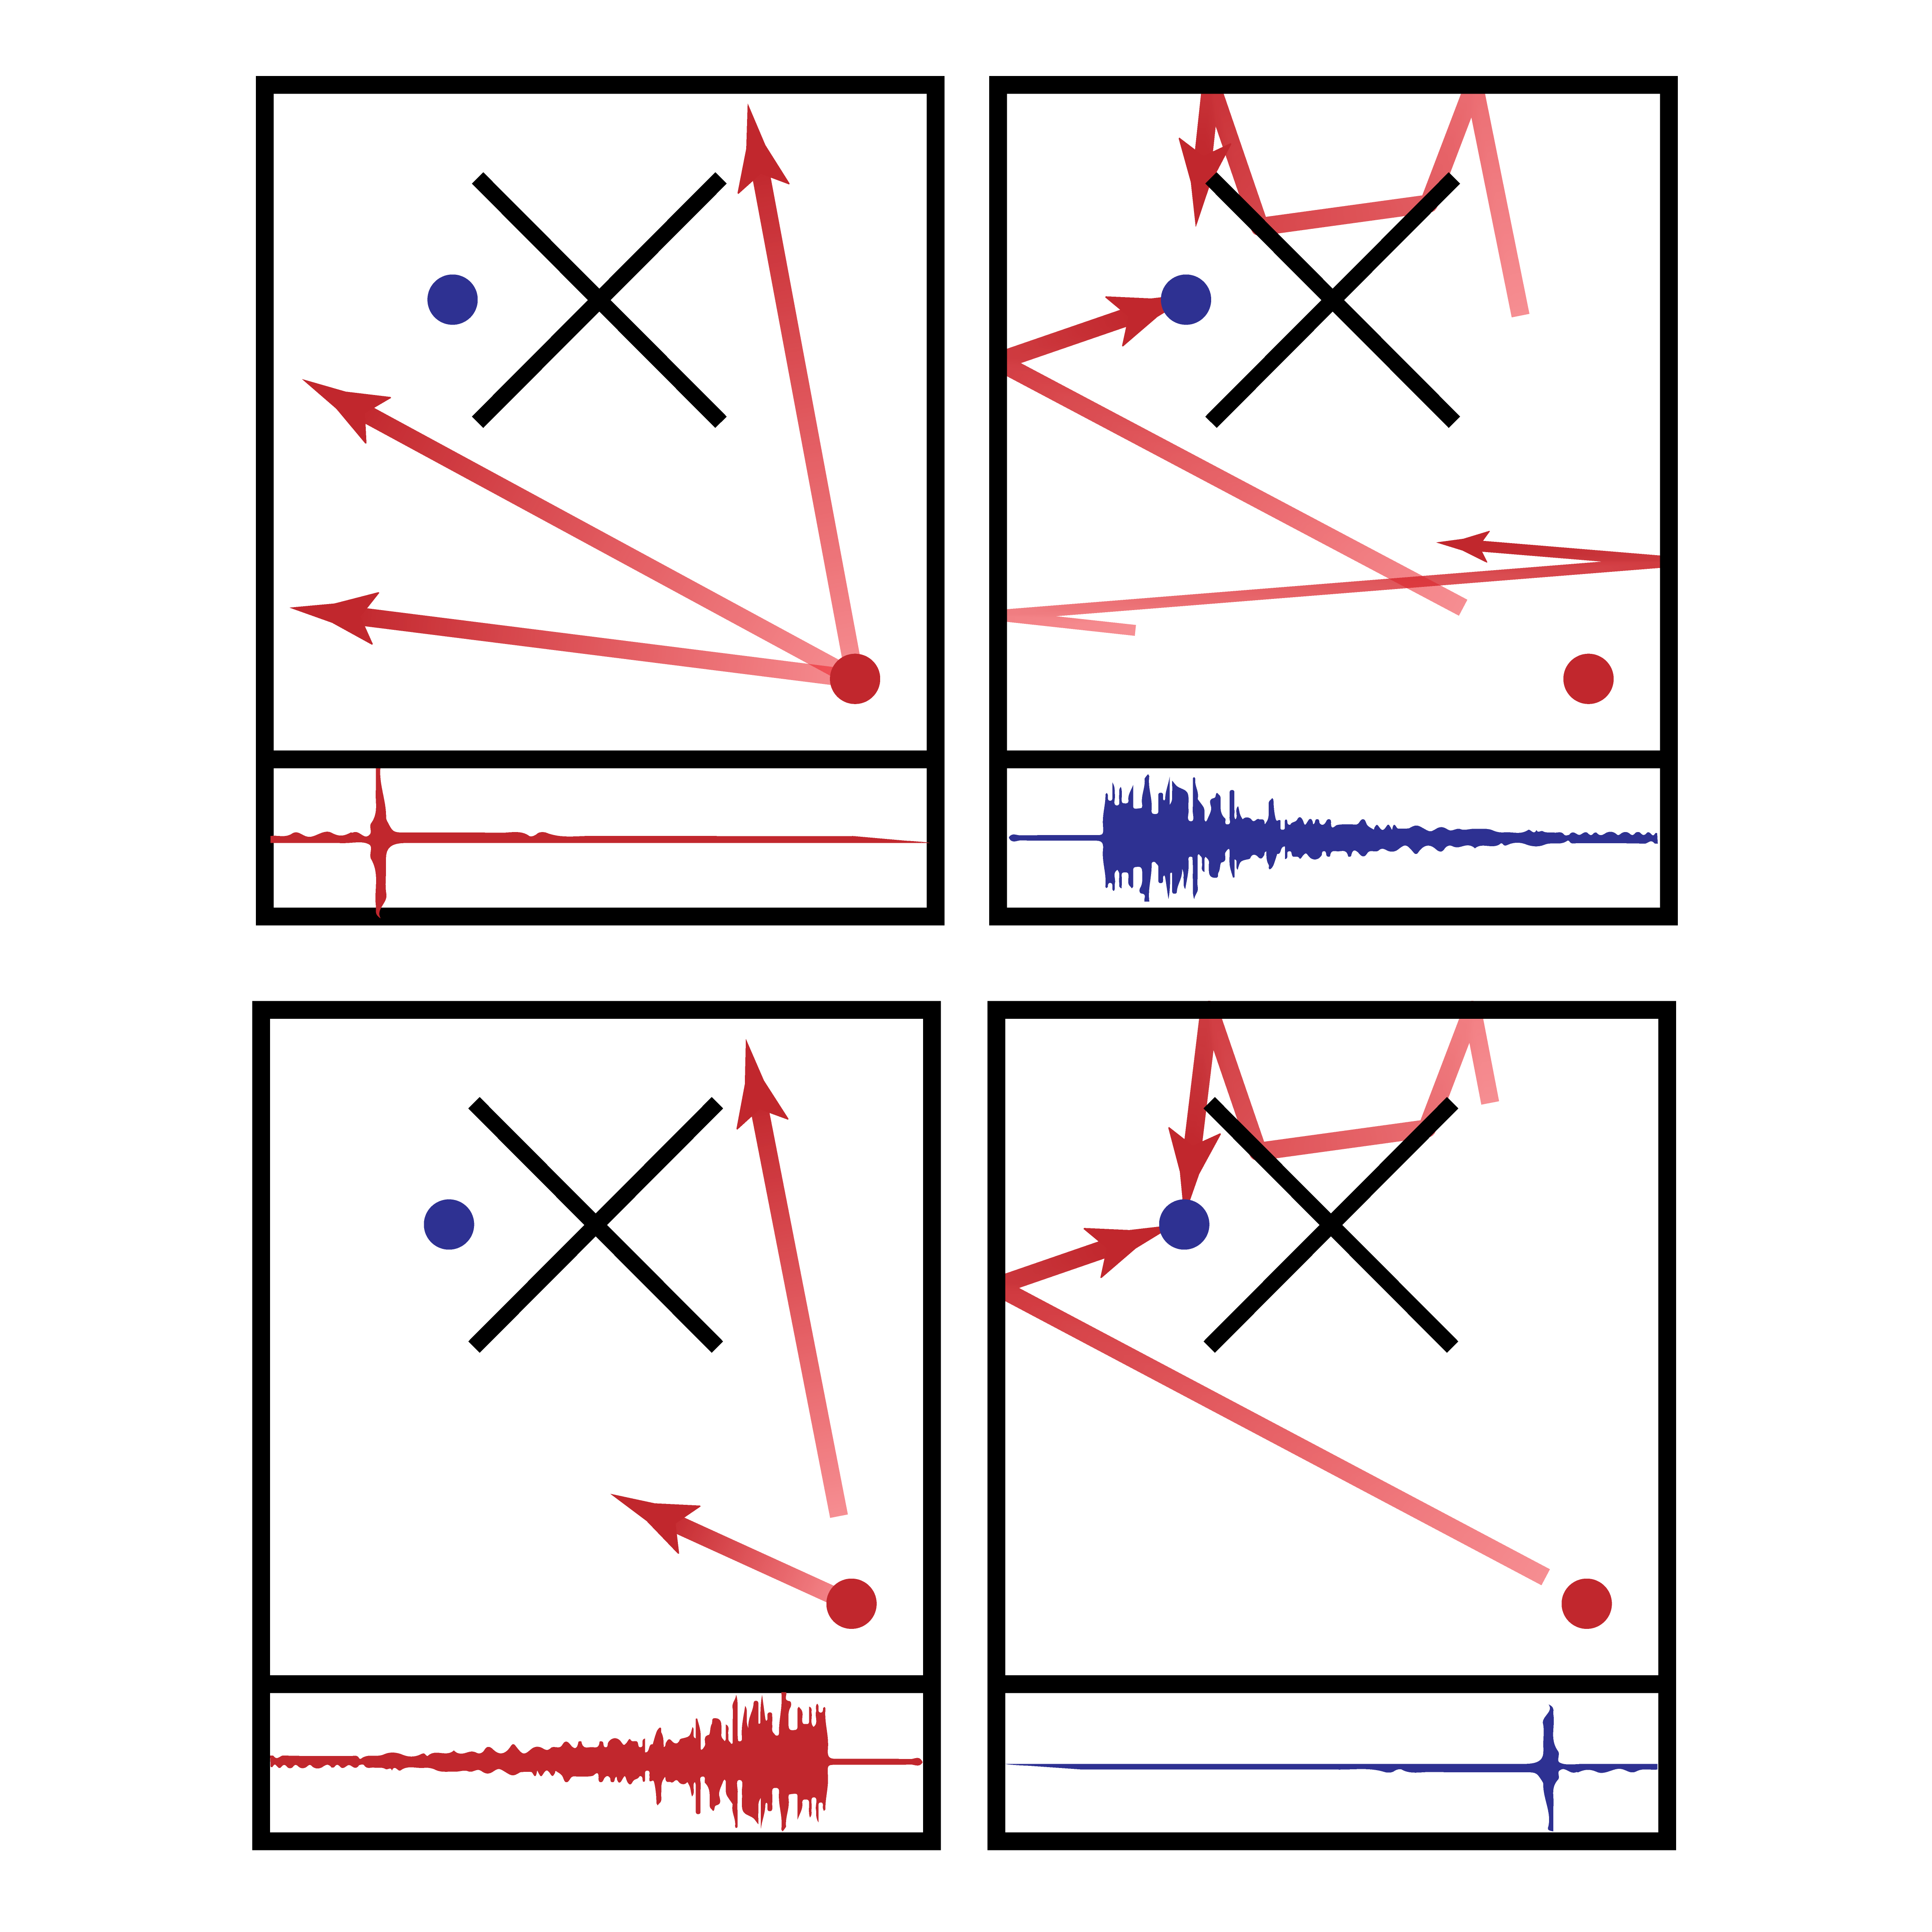
\includegraphics[width=0.85\textwidth]{linear/ltr}
    \caption[Conceptual overview of linear time reversal]{Reading order from top left: Visualization of the linear time reversal process (1) The TRM broadcasts a signal (in this case,a pulse, pictured in the inset below the panel) into the cavity, which (2) reverberates within the cavity. Some of the reflections incoherently reach the receiver as the sona, represented in blue in the inset. (3) The TRM time reverses the sona, then re-emits it into the cavity. (4) The time reversed waves coherently collapse back on the receiver in a slightly distorted reconstruction of the original pulse (inset, blue).}
    \label{fig:linear-ltr}
\end{figure}

The experiments, results, and discussions for these sections are presented in the following sections. The modifications of the basic LTR methodology as discussed and the implication for the use of TR in a WPT system. The experience the team gained by performing these experiments and formulating results was invaluable in constructing and performing our later work with Nonlinear Time Reversal (NLTR). They also demonstrate important conclusions regarding the transmission of large amounts of power to the receiver.
